\documentclass[conference]{IEEEtran}
\IEEEoverridecommandlockouts
% The preceding line is only needed to identify funding in the first footnote. If that is unneeded, please comment it out.
\usepackage{cite}
\usepackage{amsmath,amssymb,amsfonts}
\usepackage{algorithmic}
\usepackage{graphicx}
\usepackage{textcomp}
\usepackage{xcolor}
\def\BibTeX{{\rm B\kern-.05em{\sc i\kern-.025em b}\kern-.08em
    T\kern-.1667em\lower.7ex\hbox{E}\kern-.125emX}}
\begin{document}

\title{RescueBot\\


}

\author{\IEEEauthorblockN{6\textsuperscript{th} Marwa Mohammed Nabawey Hassan }
\IEEEauthorblockA{\textit{Hochschule Hamm-Lippstadt } \\
\textit{Electronic Engineering Depertment }\\
Prototyping and Systems Engineering Course \\
marwa-mohammed-nabawey.hassan@stud.hshl.de}



}


\maketitle



\begin{IEEEkeywords}
Coding, simulation, maps, programming 
\end{IEEEkeywords}




\section{Prototyping Programming}

During the programming and simulation phases, the robot starts to develop its own view of the world using  few symbols to represent each object, we have been  asked to deal with different environments and program the robot to reach its target.
In the next section, we are going to explain how we dealt with each required task, so that we end up having a robot that meet all the requirements. We have developed our code functions in C using Visual Studio Code tool. 


\subsection{Different Targets}

Throughout the  representation of  the Robot's world by a single map defined with character  array, the Robot was defined by character 'R', and asked to  reach either a land target defined by  'T' or sea target 't', and return to its home base which defined by ‘X’ after the robot leaves the initial position taking into consideration that, after the robot pick its  target the position will  turn into ‘O’ and the robot has a limitation of  maximum 200 steps. 


\begin{figure}[!h]
	
	\centering
	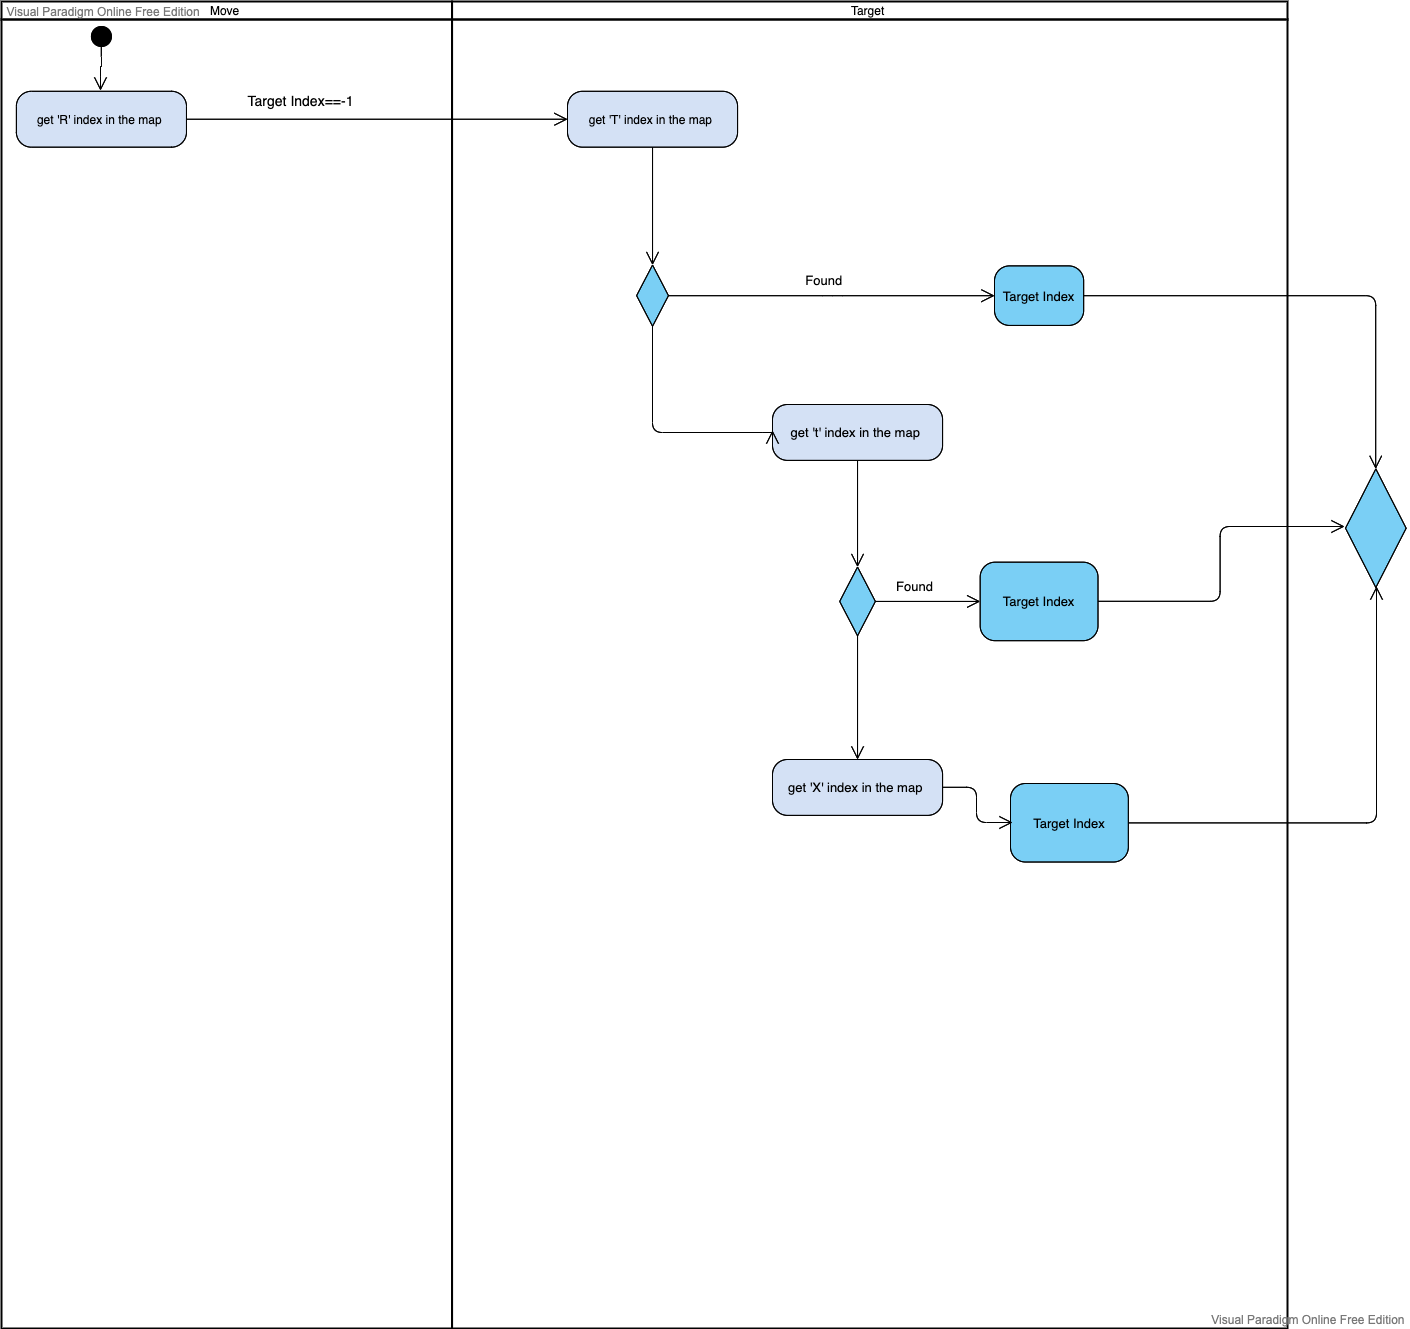
\includegraphics[width=0.4\textwidth]{targets.png}
	\caption{\label{targetAct}Different Target's Activity Diagram }
	
\end{figure}

The Fig.\ref{targetAct}   shows the activity diagram of our  approach we used to deal with different Targets.


Our approach to solve this challenge, was to initialize a Target index by "-1" after getting the Robot index in the map, the function"get\_pos" start to search for first the target 'T' if found it will then consider it as the current Target index, if  not then as next step it searches for target 't' and considered it as current target index, as a third step the function will search for the target 'X' which is the home base and considered it as the current target. Fig. \ref{targetCode}shows  the code implementation of this task. 

\begin{figure}[!h]
	
	\centering
	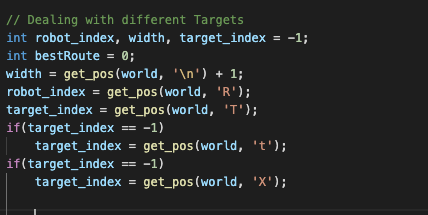
\includegraphics[width=0.4\textwidth]{targetsCode.png}
	\caption{\label{targetCode}Targets code.}
	
\end{figure}

\subsection{Avoiding Walls }

As a next task, the robot were asked to avoid crashing into walls, which is represented by '\#' , to develop that, a function ' move ' should return  an integer that represents the direction, where the robot should navigate as follows : for  North return 1,  East return 2,  South return  3
and West return  4, the Fig .\ref{wallAct} shows the activity diagram of our approach to avoid the wall.


\begin{figure}[!h]
	\centering
	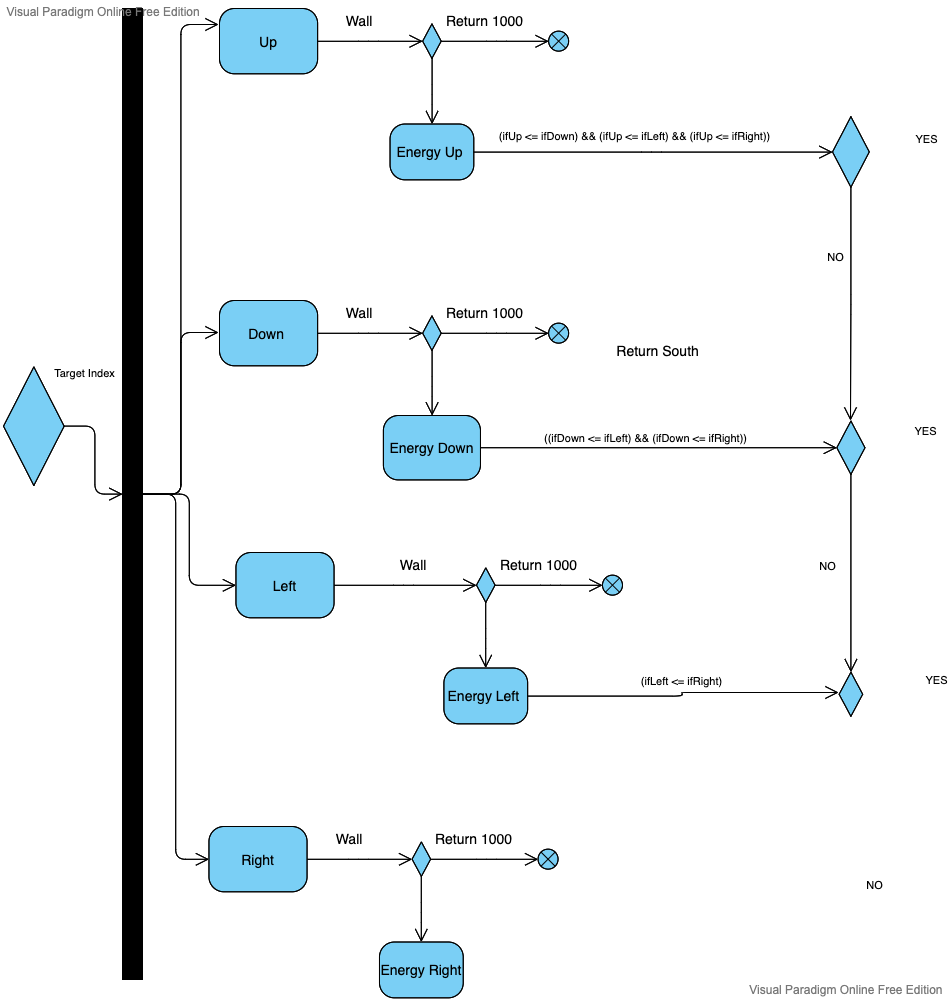
\includegraphics[width=0.4\textwidth]{wall.png}
	\caption{\label{wallAct}Avoiding walls  Activity Diagram }
	
\end{figure}


Our approach to solve this challenge, was to get  Min. steps in each direction by passing the next step to function called "minEnergy" and returning the value and store it in four variable "ifUp indicate North direction ", "ifDown for South direction ", "ifRight for East " and "IfLeft for West". The Fig.\ref{MinEnAct}shows  the activity diagram of the "minEnergy " Function. 

\begin{figure}[!h]
	
	\centering
	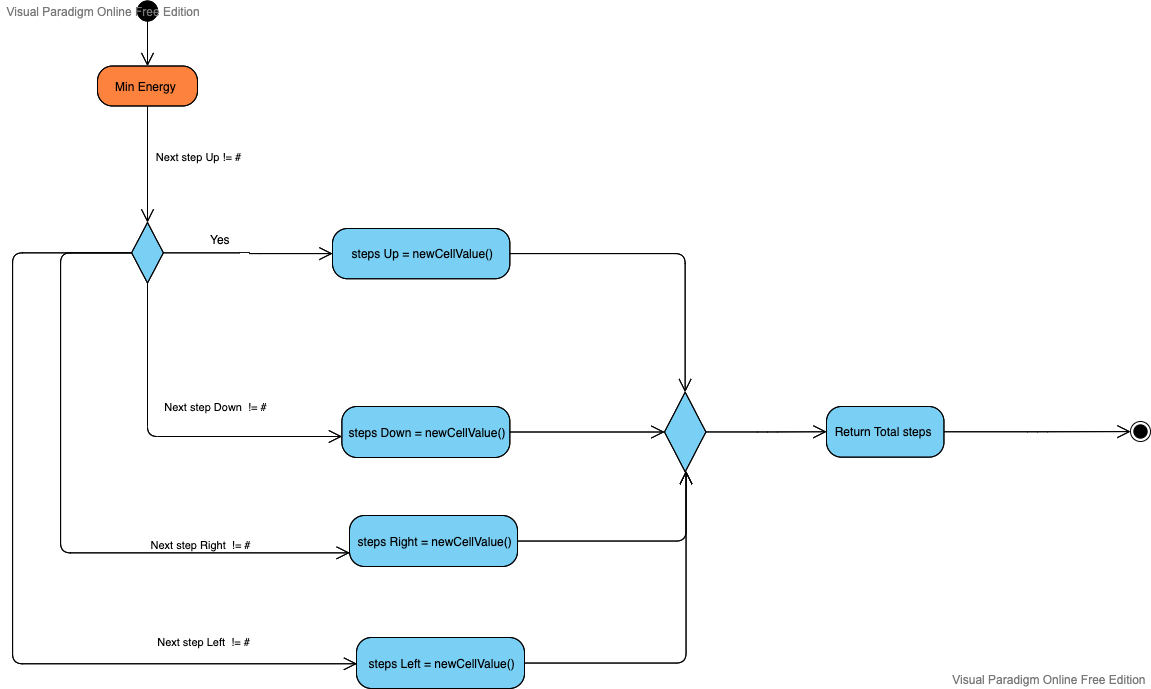
\includegraphics[width=0.4\textwidth]{MinEnergy.png}
	\caption{\label{MinEnAct}min.Energy Activity Diagram .}
	
\end{figure}



The minEnergy function check if the next potential step is wall, it will return then a '1000' which can be considered as great value, so the robot won't ever consider this direction, or the other option is that it returns the actual number of steps when taking this direction, the Fig \ref{MinEnCode} shows the code implementation of minEnergy function.


\begin{figure}[!h]
	
	\centering
	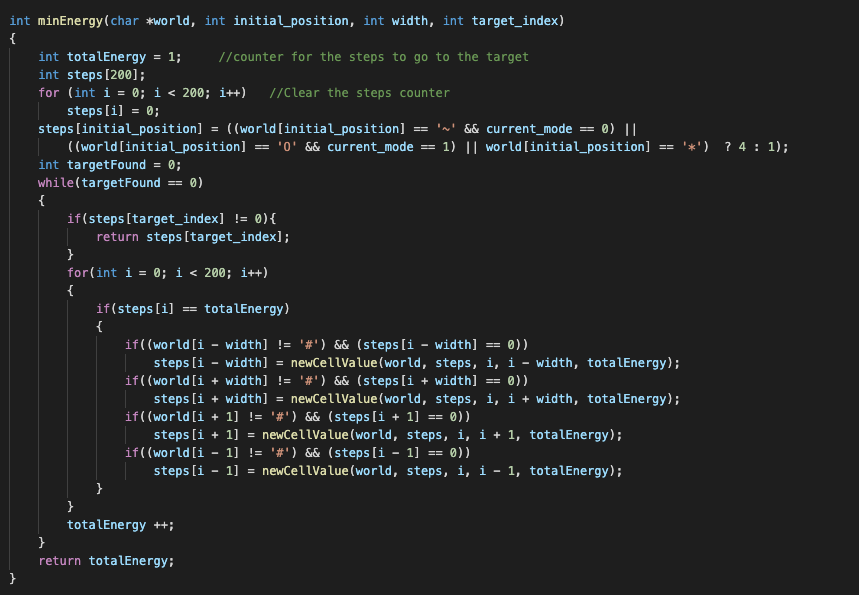
\includegraphics[width=0.4\textwidth]{MinEnergyCode.png}
	\caption{\label{MinEnCode}The implementation of minEnergy function  .}
	
\end{figure}

After the calculation  of the potential value in each direction, the values are get compared  and store in variable called "bestRoute" which hold one of the direction NORTH, SOUTH, EAST and WEST and considered it as the best route to reach the target, Fig \ref{MinstepsCode} shows the implementation of this step. 


\begin{figure}[!h]
	
	\centering
	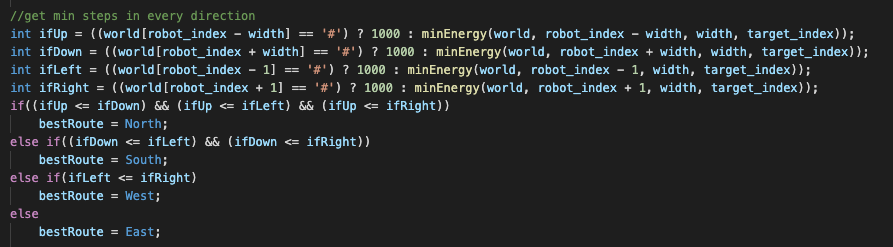
\includegraphics[width=0.4\textwidth]{minStepsCode.png}
	\caption{\label{MinstepsCode}The implementation of bestRoute  .}
	
\end{figure}



\subsection{Water Mode }


One of the Robot requirement is the ability to drive on water, which represented by  ($\sim$) symbol . To drive through water, the Robot should have to  toggle from Land to Water Mode and vice versa.  In addition to returning  1,2,3,4 to the directions  the robot should return 5 in the
move function to toggle the driving mode, the Fig.\ref{ToggleAct} shows our Approach to switch between the Two modes. 


\begin{figure}[!h]
	
	\centering
	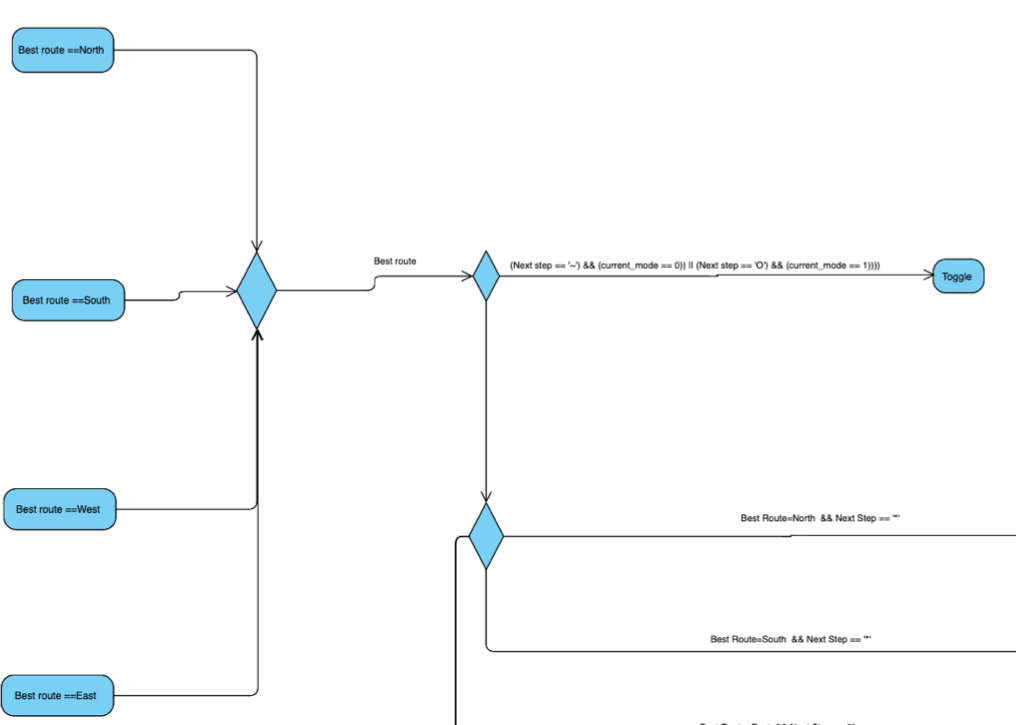
\includegraphics[width=0.4\textwidth]{Toggle.png}
	\caption{\label{ToggleAct}Activity diagram of Toggle scenario  .}
	
\end{figure}


After the best route is defined, the move function check if the next step is water and the current mode is Land, and return a Toggle. As well as checking the other scenario if the next step is land and the current mode is water, it will toggle the mode. The Fig.\ref{ToggleCode} shows the code implementation of this task.


\begin{figure}[!h]
	
	\centering
	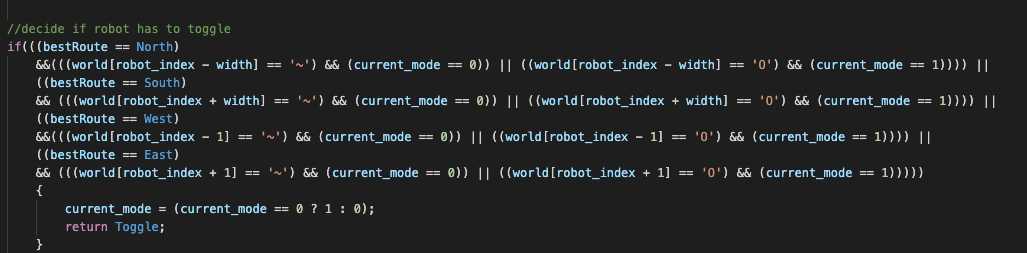
\includegraphics[width=0.4\textwidth]{ToggleCode.png}
	\caption{\label{ToggleCode}The implementation of Toggle scenario  .}
	
\end{figure}


\subsection{ Dealing with Obstacles}

As a last Task the Robot's world gets more complicated to consider new barriers, beside the Wall the map will contain  obstacles described with  (‘*’) symbol, that can be destroyed, The robot will consume  energy based on  10 unit energy per movement,  30 unit energy per toggle and  70 unit energy for trying to destroy an obstacle, and we will have to use min Energy to fulfill the task. 

In addition, if we choose to destroy the  obstacle, the function will return a new value as  6 to  destroy an obstacle to the north, 7 to destroy an obstacle to the east,8 to destroy an obstacle to the south and  9 to destroy an obstacle to the west. The Fig. \ref{ObstAct} shows our approach to solve this task .

\begin{figure}[!h]
	
	\centering
	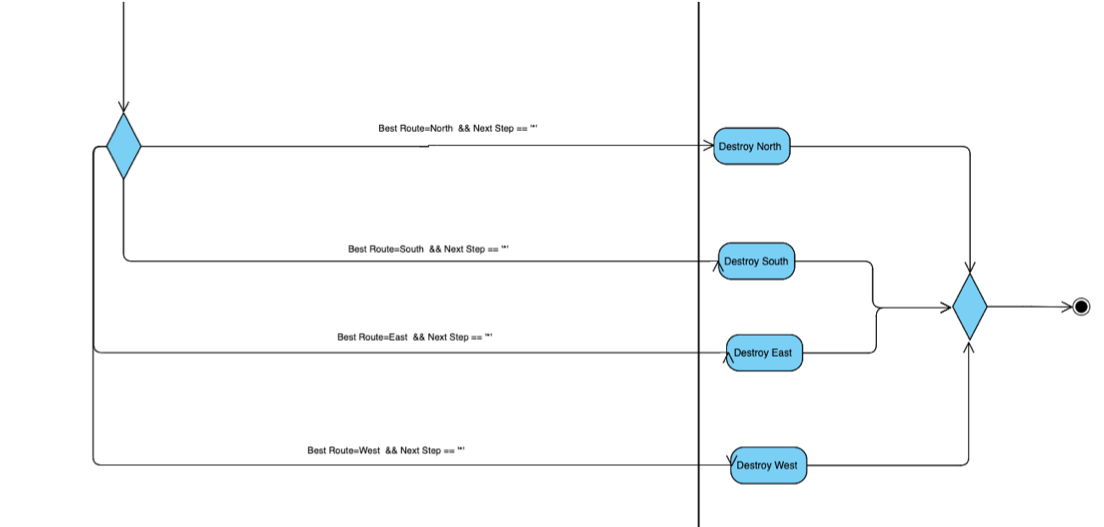
\includegraphics[width=0.4\textwidth]{Obstecles.png}
	\caption{\label{ObstAct}Activity diagram of dealing with obstecles  .}
	
\end{figure}


After getting the best route, the function newCellValue will return either Energy+ 1, when they meet any Target, or Energy+4, if  it faces any Obstacle in any direction or if faces a water or land, when need to toggle. The fact that it will return only 4 when destroying an obstacle, because the robot will consume only one time the amount of energy to destroy the obstacles in  the two-way path. The Fig.   \ref{nextstepAct} shows the activity diagram of newCellValue and how it returns either Energy+1 or Energy+4. 

\begin{figure}[!h]
	
	\centering
	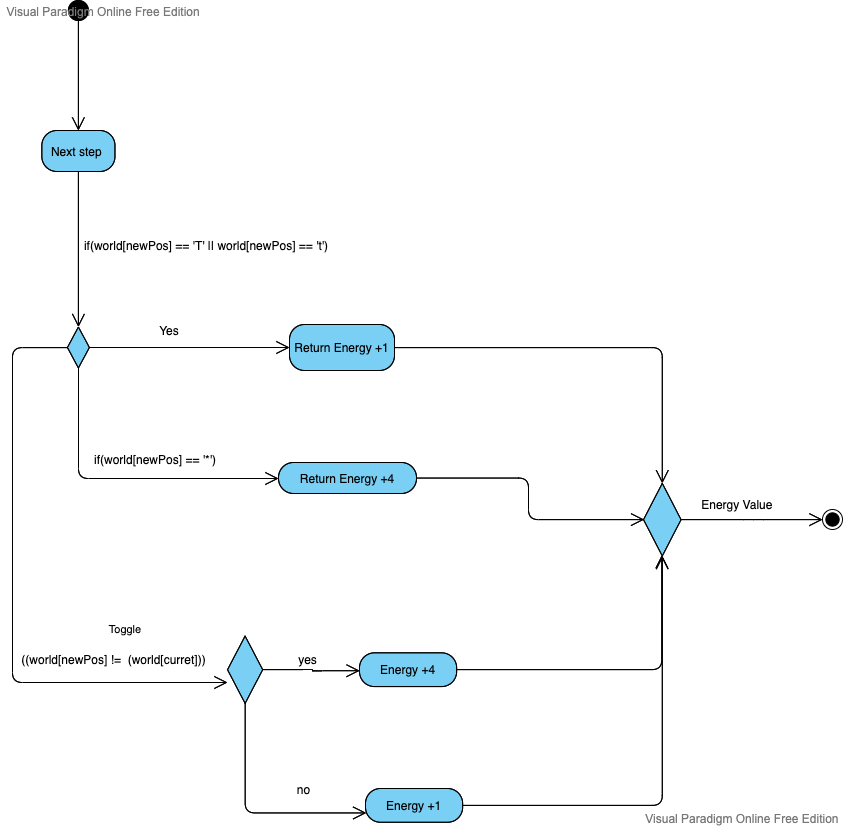
\includegraphics[width=0.4\textwidth]{NextStep.png}
	\caption{\label{nextstepAct}Activity diagram of newcellValue function .}
	
\end{figure}



The implementation of the function is shown in Fig. \ref{calCode}


\begin{figure}[!h]
	
	\centering
	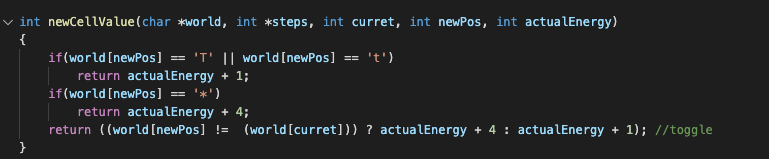
\includegraphics[width=0.5\textwidth]{newCalCode.png}
	\caption{\label{calCode} Implementation of newcellValue function .}
	
\end{figure}


After getting the best route and the potential next step contains any obstacle, the function  will then return to destroy in this direction to deal with the obstacle. The checking of conditions is done in four direction North, South, East, west, If the robot's best route doesn't contain any obstacles, it will send then the best Route. The Fig. \ref{obstCode} shows the code implementation when destroying obstacle. 

\begin{figure}[!h]
	
	\centering
	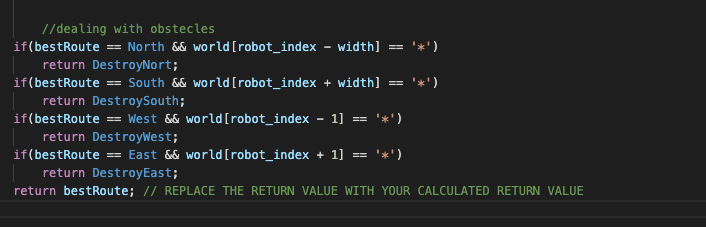
\includegraphics[width=0.4\textwidth]{oBSTECLEScODE.png}
	\caption{\label{obstCode} Implementation of destroying obstacles scenario  .}
	
\end{figure}





\end{document}
